% !TEX root = report.tex

\section{Processing Pipeline}
\label{sec:processing_architecture}

High level descripion of the processing flow:

Throughout the report: extract Spectrograms, classify image.

\section{Signals and Features}
\label{sec:model}

\subsection{Google Dataset}

% Measurement setup, data preprocess (describe the google dataset)

The Speech Commands datasets, described in \cite{warden2018speech}, provides
thousands of one second recording of $35$ differen words. The recordings are
mainly of volounteers, who used their own device to record the words in a
closed room wherever they happened to be (not in a studio setting).
Ideally each volounteer only recorded the $135$ requested utterances once, so the
dataset provides good variability of voices.
The utterances have a duration of one second.
To more precisely align the recorded clips, the audio was acquired for $1.5$
seconds and the $1$ second clip that contained the highest overrall volume was
extracted.
Several background noise recording are included as well.
The full dataset includes $105829$ utterances of $35$ words, saved in
\textit{.wav} format at $16$ KHz rate.
The dataset is released under the Creative Commons BY $4.0$ License \cite{ccby4}.

The dataset ships with a function to split the data in train, validation and
test folds, as well as two example lists of validation data ($9981$ utterances)
and test data ($11005$ utterances).
Throughout the experiments, those lists were used.
% both for the practicality of having them ready, but also to keep with the
% spirit of the dataset as a tool to enable meaningf

TODO: how the words are grouped

\subsection{Mel spectrogram and Mel-frequency Cepstral Coefficients}

The audio data in the dataset is available as a vector of amplitudes over time,
sampled at $16$ KHz. In this representation, the classification task is quite
hard.
The Fourier transform allows to convert a signal from the time domain into the
frequency domain. The result is called spectrum of the signal. This transform
is efficiently computed using the Fast Fourier Transform algorithm.

The short-time Fourier transform accounts for variations of the content of an
audio signal over time. Instead of computing the FFT of the entire signal, the
FFT is computed on overlapping windowed segments of the signal: each window has
length \texttt{n\_fft} and the next window is extracted after
\texttt{hop\_length} samples.
The results of the FFT in each window are stacked to obtain the spectrogram.

The human ear does not perceive frequencies on a linear scale: the difference
between $200$ and $400$ Hz is very marked, whereas two notes at $8000$ and
$8200$ Hz are almost indistinguishable. The mel scale, proposed by Stevens,
Volkmann, and Newmann \cite{melscale1937}, introduces a unit of pitch built in
such a way that equal distances on the scale sound equally distant to the human
listener.
The mel spectrogram is a spectrogram where the frequencies are converted to the
mel scale. To do so, a Mel spaced filterbank is generated (a 10 filters version
is shown in \fig{fig:mel10_filterbank}) and the FFT results are multiplied with
a dot product with each filter, obtaining \texttt{n\_mel} values for each
timestep.

\begin{figure}[t!]
    \centering
    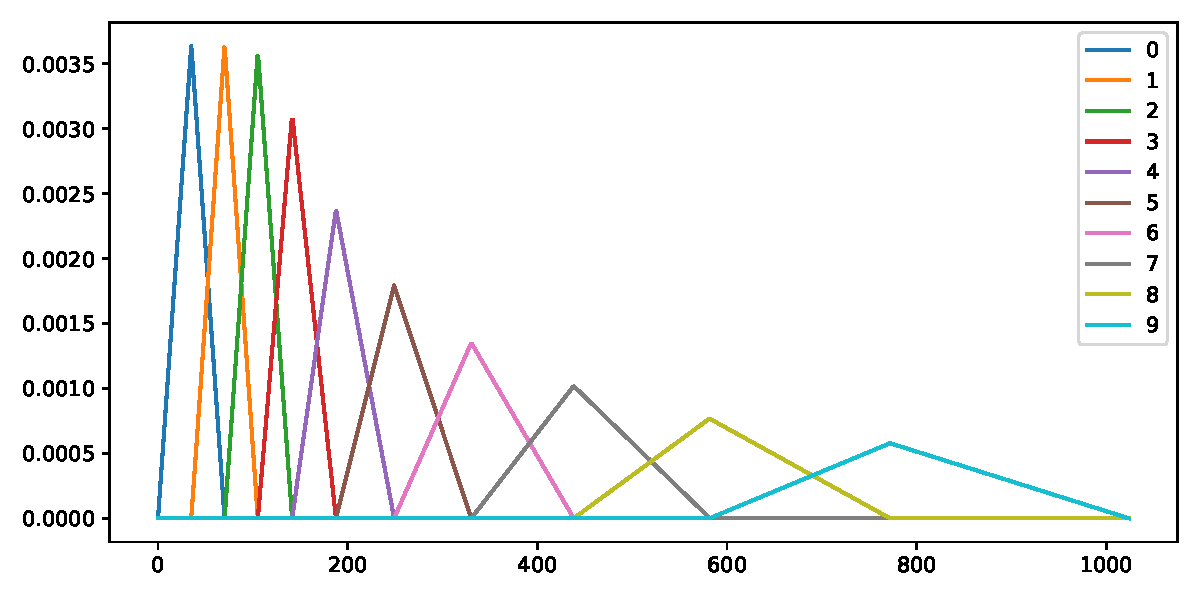
\includegraphics[width=0.8\linewidth]{mel10_filterbank.pdf}
    \caption{An example of a 10 filters Mel filterbank}
    \label{fig:mel10_filterbank}
\end{figure}

The resulting coefficients are highly correlated: the Discrete Cosine Transform
can be applied to decorrelate the filter bank coefficients and obtain a
compressed representation.
The results are the Mel-frequency Cepstral Coefficients.

The spectrograms were obtained using the \texttt{librosa} library \cite{brian_mcfee_2020_3955228}.
The values used to generate the mel spectrograms are listed in
\tab{tab:mel_values}.
The values used to generate the mel frequency cepstral coefficients are listed
in \tab{tab:mfcc_values}.
An example waveform for the word ``happy'' and the relative spectrograms are
shown in \fig{fig:happy_specs}.

\begin{figure}[t!]
    \centering
    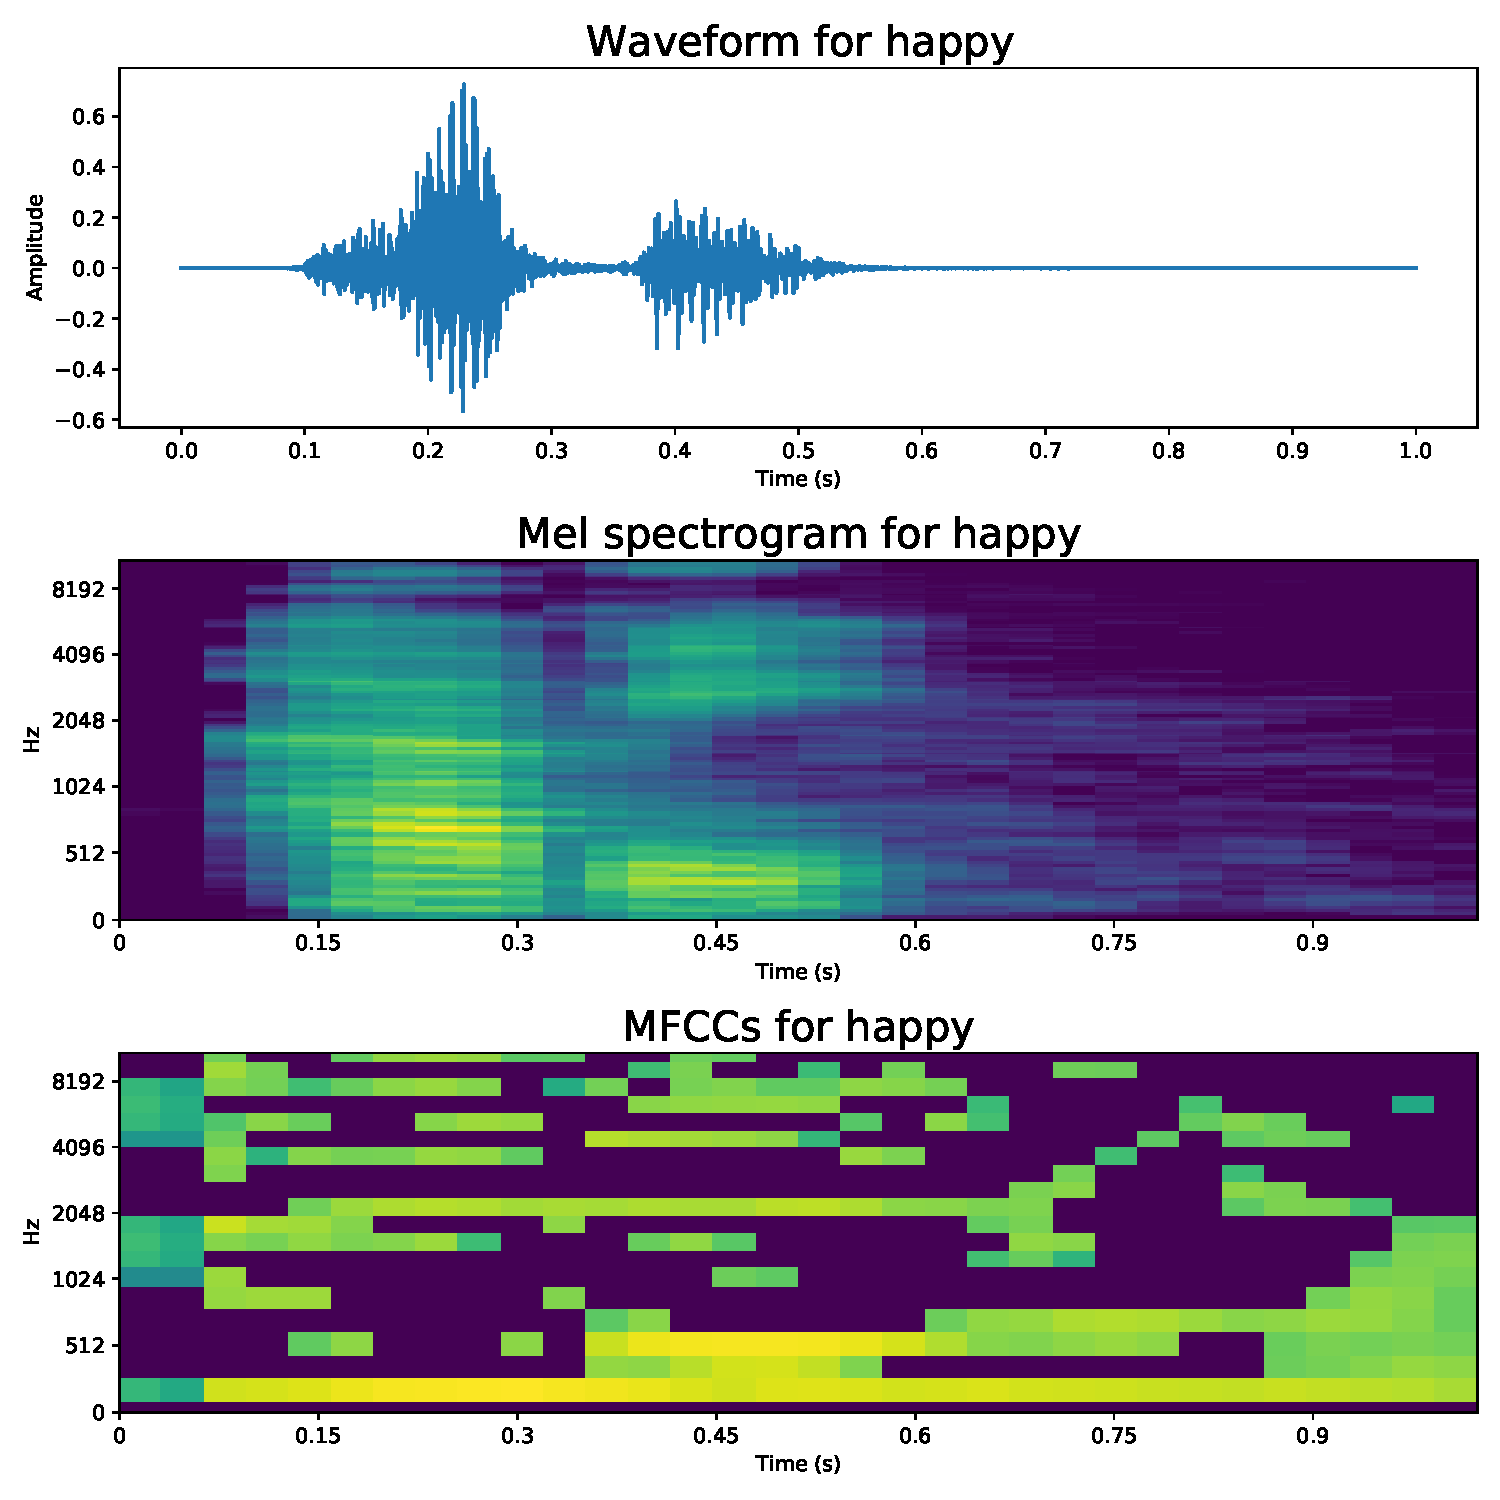
\includegraphics[width=0.8\linewidth]{happy_specs.pdf}
    \caption{
    Waveform and spectrograms for the word happy. Note that the y axis of the
spectrograms are labeled as Hz, but this is only to read more easily the plot
and understand to which frequencies the important bins correspond to. }%
    \label{fig:happy_specs}
\end{figure}

\begin{table}[t!]
    \centering
    \caption{
    Values used to generate the mel spectrograms. The dataset ``mela1'' also
has the parameter \texttt{fmin}$=40$.}
    \label{tab:mel_values}
    \begin{tabular}{|c|cccc|}
        \hline
        % name & \texttt{n\_mel} & \texttt{n\_fft} & \texttt{hop\_length} & shape \\
        name & n\_mel & n\_fft & hop\_length & shape \\
        \hline
        mel01 & 128 & 2048 & 512   & (128, 32) \\
        mel02 & 64  & 4096 & 1024  & (64, 16) \\
        mel03 & 64  & 2048 & 512   & (64, 32) \\
        mel04 & 64  & 1024 & 256   & (64, 64) \\
        mel05 & 128 & 1024 & 128   & (128, 128) \\
        mel06 & 128 & 1024 & 256   & (128, 64) \\
        mel07 & 128 & 2048 & 256   & (128, 64) \\
        mel08 & 128 & 512  & 256   & (128, 64) \\
        mel09 & 128 & 512  & 128   & (128, 128) \\
        mel10 & 128 & 2048 & 128   & (128, 128) \\
        mel11 & 128 & 256  & 128   & (128, 128) \\
        mel12 & 128 & 4096 & 256   & (128, 64) \\
        mel13 & 128 & 512  & 256   & (128, 64) \\
        mel14 & 128 & 256  & 256   & (128, 64) \\
        mel15 & 128 & 3072 & 256   & (128, 64) \\
        mela1 & 80  & 1024 & 128   & (80, 128) \\
        \hline
    \end{tabular}
\end{table}

\begin{table}[t!]
    \centering
    \caption{Values used to generate the MFCC spectrograms}
    \label{tab:mfcc_values}
    \begin{tabular}{|c|cccc|}
        \hline
        % name & \texttt{n\_mfcc} & \texttt{n\_fft} & \texttt{hop\_length} & shape \\
        name & n\_mfcc & n\_fft & hop\_length & shape \\
        \hline
        mfcc01 & 20  & 2048 & 512  & (20, 32) \\
        mfcc02 & 40  & 2048 & 512  & (40, 32) \\
        mfcc03 & 40  & 2048 & 256  & (40, 64) \\
        mfcc04 & 80  & 1024 & 128  & (80, 128) \\
        mfcc05 & 10  & 4096 & 1024 & (10, 16) \\
        mfcc06 & 128 & 1024 & 128  & (128, 128) \\
        mfcc07 & 128 & 512  & 128  & (128, 128) \\
        mfcc08 & 128 & 2048 & 128  & (128, 128) \\
        \hline
    \end{tabular}
\end{table}

TODO: composing datasets, multichannel

\subsection{Data augmentation}

Data augmentation is a technique to increase the amount of data available by
applying random, but meaningful, transformations to the data. This leads to a
noisier dataset, that should make the trained model more robust and less prone
to overfitting. The data was augmented both by modifying the waveform and the
spectrograms. An option to include the originals in the augmente dataset is
available.

\subsubsection{Time shift}

The waveform is shifted by a random amount of samples, controlled by the
parameter \texttt{max\_time\_shift}.

\subsubsection{Time stretch}

The waveform is stretched, making the sound slower or faster, controlled by the
parameter \texttt{stretch\_rate}.

\subsubsection{Spectrogram warp}

The spectrogram is warped using the \texttt{sparse\_image\_warp} function
available as a tensorflow addon.
A sequence of source landmarks is randomly selected within the image, and the
points are shifted by a random amount along both time and frequency axis. The
warp is controlled by the parameters \texttt{num\_landmarks},
\texttt{max\_warp\_time} and \texttt{max\_warp\_freq}.
The effect of warping an image is shown in \fig{fig:warp_grid}.

Several augmentations were performed, mostly focussing on the spectrogram
warping, along one or both time and frequency axis.
Values used to augment the dataset are listed in \tab{tab:aug_values}.

\begin{figure}[t!]
    \centering
    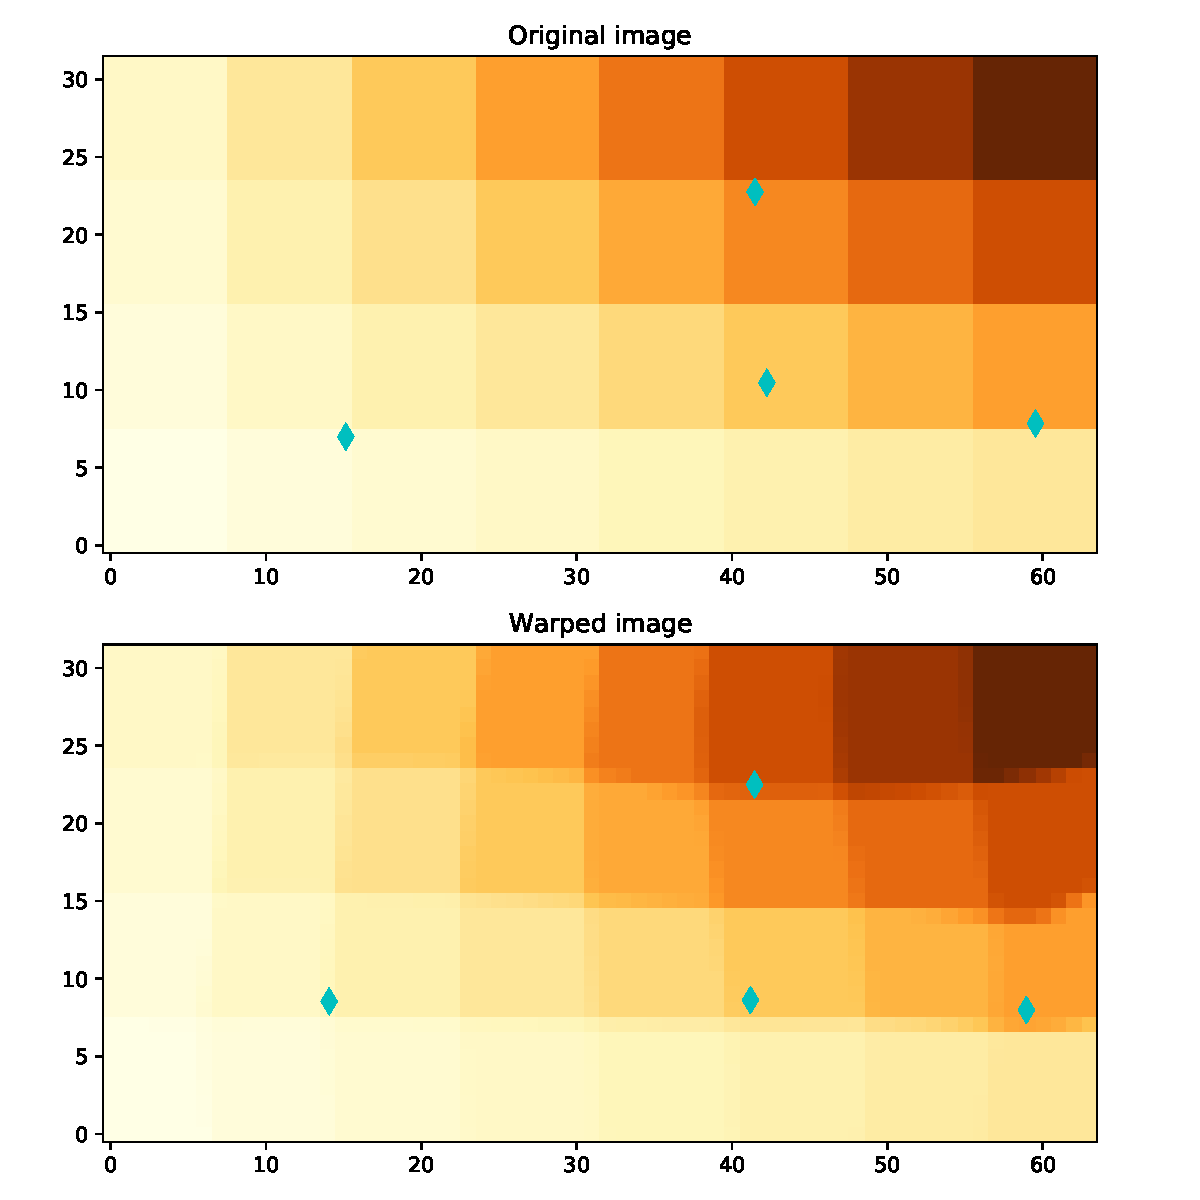
\includegraphics[width=0.8\linewidth]{warp_grid.pdf}
    \caption{
    The effects of \texttt{sparse\_image\_warp} on an image, with
\texttt{num\_landmarks} $=4$, \texttt{max\_warp\_time} $=2$ and
\texttt{max\_warp\_freq} $=2$. The diamonds show the source and destination
landmarks.}%
    \label{fig:warp_grid}
\end{figure}

\begin{table*}[t!]
    \centering
    \caption{Values used to augment the dataset. The first lines list the parameters used to compute the spectrograms.}
    \label{tab:aug_values}
    \begin{tabular}{|c|cccccc|}
        \hline
        & mel\_kwargs & n\_mel & n\_fft & hop\_length & fmin & fmax \\
        \hline
        & mel\_01 & 64 & 1024 & 256 & 40 & 8000  \\
        & mel\_02 & 128 & 2046 & 512 & 40 & 8000  \\
        & mel\_03 & 64 & 1024 & 256 & default & default  \\
        \hline
        \hline
        aug name & max\_time\_shifts & stretch\_rate & mel\_kwargs & num\_landmarks & max\_warp\_time & max\_warp\_freq\\
        \hline
        aug01 &  [1600, 3200] & [0.8, 1.2] & mel\_01 & 3 & 5 & 6 \\
        aug02 &  [] & [] & mel\_02 & 3 & 5 & 5 \\
        aug03 &  [] & [] & mel\_02 & 3 & 5 & 0 \\
        aug04 &  [] & [] & mel\_02 & 3 & 0 & 5 \\
        aug05 &  [] & [] & mel\_02 & 3 & 0 & 0 \\
        aug06 &  [] & [] & mel\_01 & 3 & 5 & 5 \\
        aug07 &  [] & [] & mel\_01 & 3 & 5 & 0 \\
        aug08 &  [] & [] & mel\_01 & 3 & 0 & 5 \\
        aug09 &  [] & [] & mel\_01 & 3 & 0 & 0 \\
        aug10 &  [] & [] & mel\_03 & 3 & 5 & 5 \\
        aug11 &  [] & [] & mel\_03 & 3 & 5 & 0 \\
        aug12 &  [] & [] & mel\_03 & 3 & 0 & 5 \\
        aug13 &  [] & [] & mel\_03 & 3 & 0 & 0 \\
        \hline
    \end{tabular}
\end{table*}

\section{Learning Framework}
\label{sec:learning_framework}

How did it learn anything at all?

\subsection{Learning rate schedule}

\subsubsection{Fixed LR}
\subsubsection{Exp decay LR}
\subsubsection{Cyclic LR}

\subsection{Early stopping}

Loss, validation, overfitting

Show a plot

\subsection{Hyper-parameter tuning}

Come lo fai

Usare Pool

Ovviamente non su tutte le combinazioni

Epoche/batch, tempo di computazione

\section{Convolutional Neural Network}
\label{sec:convolutional_arch}

\subsection{Architecture}

As a starting benchmark, a standard Convolutional Neural Network was implemented.
Three convolutional modules are instantiated, followed by a dense classifier.
Each convolutional module is composed of the convolutional layer, a batch
normalization layer, a max pooling layer and a dropout layer.
The classifier is composed by three dense layers, the last with softmax
activation and a number of units equal to the number of classes to predict.

\subsection{Model hyper-parameters}

When building the model, aside from the number of classes to predict and the
input shape of the spectrogram, five parameters can be set:
\begin{enumerate}
    \item Number of convolutional filters: deeper layers have to learn more
        filters, as the feature maps decrease in width and height after the
        pooling.
    \item Shape of the convolutional filters:
        both square and rectangular filters were tested.
        A vertical rectangular filters (e.g. (5, 1)) emphasizes the
        relationship between mel coefficients within the same time step
    \item Shape of the pooling window: 
        both square and rectangular windows were tested.
        Again, a rectangular filter allows to push into deeper layers more
        information along the time or frequency axis.
    \item Dropout rates after the convolutional modules.
    \item Width of the dense classifier layers.
\end{enumerate}
The possible values for the hyper-parameters are:
\begin{itemize}
    \item dense\_width = [16, 32, 64, 128]
    \item filters = [10, 20, 32, 64, 128]
    \item dropout = [[0.03, 0.01],  [0.3, 0.1]]
    \item kernel\_size = [[(2,2), (2,2), (2,2)], [(5,1), (3,3), (3,3)]]
    \item pool\_size = [[(2,2), (2,2), (2,2)], [(2,1), (2,2), (2,2)]]
\end{itemize}

% hypa_grid['dataset'] = ['mfcc01' 'aug13' 'mel01' 'aug02' 'mfcc03' 'aug07' 'aug04' 'mel03'
%  'mfcc04' 'mfcc02' 'mel04' 'aug10' 'aug03' 'mel02' 'aug06' 'aug05' 'mela1'
%  'aug09' 'aug08' 'aug12' 'aug11' 'aug14' 'aug15']
% hypa_grid['words'] = ['f1' 'num' 'k1' 'w2' 'f2' 'all' 'dir']

% hypa_grid['batch_size'] = [128  32  64]
% hypa_grid['epoch_num'] = [ 60  15  16  30  59  58  61  31  62 101]
% hypa_grid['lr'] = ['default' '01' '03' '02' '06' '04' '05' 'e1']
% hypa_grid['opt'] = ['adam' 'a1' 'r1']


\section{Transfer Learning Approach}
\label{sec:transfer_learning}

\subsection{Transfer learning}

Transfer learning is a technique where a model developed and trained for a task
is modified slightly and used as a starting point for a different task.
A Convolutional Neural Network can be seen as a feature extractor composed with
a classifier.
The feature extractor is the largest part of the network, consisting in roughly
90\% of the trainable weights.
The idea behind transfer learning is to leverage the knowledge acquired
regarding the first part, extracting meaningful features from an image, and
modifying the latter, re-learning the classifier.
Training these big networks (10-100 millions of parameters) on ImageNet (14
millions of images in 1000 classes) can take from days to over a month even on
supercomputers with dozens of top of the line graphics cards.
Adapting the networks for a new task, on the other hand, is a matter of roughly
half an hour on a single GPU.

As spectrograms can be interpreted as images, starting from an image classifier
makes perfect sense. The two architecture used are Xception 
\cite{chollet2017xception}
and EfficientNet
\cite{tan2020efficientnet}.

\subsubsection{Xception structure}

A standard convolutional layer tries to learn 3D filters, with two spatial
dimensions and one channel dimension.
Such a filter has to simultaneously learn spatial correlations and
cross-channel correlations.
The Inception Hypothesis asserts that it would be easier to learn independently
the cross-channel and spatial correlations.
To do so an Inception module first learns cross-channel correlations with 1x1
convolutions, then learns spatial correlations with standard 3x3 and 5x5
convolutions.
The Xception model pushed this hypothesis to the limit, completely decoupling
the mapping of spatial and cross-channel correlations.

\subsubsection{EfficientNet structure}

Scaling a Convolutional Neural Network can lead to increased performance:
adding more layers, more filters of more convolutional modules can make the
model more accurate. On the other hand, a bigger model means slower training
and higher memory consumption to the point of being infeasible to train.
On top of that, often CNN can be over-parametrized: model compression
techniques can trade little accuracy for a great reduction in model size
\cite{han2016deep}.

The EfficientNet authors carefully examine the scaling of a model to obtain the
optimal parameters of width, depth and resolution, proposing a new compound
scaling method, which uses a single compound coefficient to scale the three
parameters in a coordinated way.
% which use a compound coefficient φ to uniformly scales network width, depth,
% and resolution in a principled way we have also developed a new mobile-size
% baseline, called EfficientNet fix φ = 1, assuming twice more resources
% available, and do a small grid search of α, β, we then fix α, β, γ as
% constants and scale up baseline network with different φ

\subsection{Transfer learning and fine tuning}

The pipeline to train a model using transfer learning is as follows:
\begin{enumerate}
    \item Load a previously trained base model, without the final classifier.
    \item Freeze the base model weights, to avoid destroying the information they
        contain.
    \item Add a classifier on top of the base model.
    \item Train the classifier, using a reasonably high learning rate.
    \item Un-freeze the base model weights.
    \item Train the model again, with a very small learning rate, to fine tune
        the feature extractor to the current dataset.
\end{enumerate}

The first four steps are the transfer learning part, followed by the fine
tuning steps five and six.

\subsection{Model building and hyper-parameters}

The inputs to the pre-trained Xception and EfficientNet models have to be
normalized, which can be easily done with a Normalization layer provided by
tensorflow.
It is to note that the inputs should be of shape $\left( 299, 299, 3 \right)$,
whereas the spectrograms used were of size $\left( 128, 128, 3 \right)$, so
some loss of performance can be expected.
The classifier built is composed by a GlobalAveragePooling2D layer, which
averages the values in each feature extracted, followed by some dense layers
(according to the hyper-parameters selected) and finally a softmax layer to
compute the predictions.

When building the model, aside from the number of classes to predict and the
input shape of the spectrograms, two parameters can be set:
\begin{enumerate}
    \item Dropout rate after the GlobalAveragePooling2D layer.
    \item Dense width and number of the dense layers in the classifier.
\end{enumerate}
The possible values for the hyper-parameters are:
\begin{itemize}
    \item dropout\_types = [0.2, 0.1, 0]
    \item dense\_width\_types = [[4, 0], [16, 16], [0, 0], [64, 64]]
\end{itemize}
Where a value of $0$ means that the layer is skipped.

\section{Attention Model}
\label{sec:attention_model}

\subsection{Attention architecture}

The key idea behind the Attention mechanism is the assumption that not all of
the data carries the same amount of information.
Indeed, when processing a large amount of information we focus on few relevant
details.
This approach was used effectively in the field of Neural Machine Translation by
Bahdanau \cite{bahdanau2016neural}
and
Luong \cite{luong2015effective}, and to produce image captions with the 
Show, Attend and Tell approach \cite{xu2016show}.

In the paper by Douglas et al. \cite{2018arXiv180808929C}, the attention
mechanism is used for speech command recognition.
As a first step, the mel spectrogram is computed from the input audio.
A 2D convolution is performed, only along the time axis to extract local
correlations in the spectrogram.
Two bidirectional \cite{Schuster1997BidirectionalRN} long short-term memory
\cite{lstm} units are used to capture forward and backward long term
dependencies in the spectrogram.
A LSTM unit reads the input sequence from the first sample to the last. The
bidirectional version reads the sequence both forward, producing the forward
hidden states, and backward, resulting in the sequence of backward hidden
states.
Here the attention mechanism is applied: one of the LSTM output vector is
selected (the choice is not crucial because the vectors should contain
information about long term dependencies) and a dense layer is used to extract
a query vector.
The query vector is then used to compute the attention scores, that are
converted with a softmax layer in attention weights. These weights are
multiplied with the output of the LSTM to compute a weighted average, which is
then fed into a dense classifier.

% https://towardsdatascience.com/an-introduction-to-attention-transformers-and-bert-part-1-da0e838c7cda
% In the proposed model, each generated output word is not just a function of
% just the final hidden state but rather a function of ALL hidden states. And,
% it’s not just a simple operation that combines all hidden state — if it was,
% then we are still giving the same context to every output step, so it has to be
% different! It is not a simple concatenation or dot product, but an “attention”
% operation that, for every decoder output step, produces a distinct vector
% representing all encoder hidden states but giving different weights to
% different encoder hidden state.

% https://arxiv.org/pdf/1409.0473.pdf
% reads an input sequence x in order starting from the first symbol x1 to the
% last one xTx . However, in the proposed scheme, we would like the annotation
% of each word to summarize not only the preceding words, but also the
% following words. Hence, we propose to use a bidirectional RNN The forward RNN
% −→f reads the input sequence as it is ordered (from x1 to xTx) and calculates
% a sequence of forward hidden states ( −→h 1, · · · , −→h Tx). The backward
% RNN ←−f reads the sequence in the reverse order (from xTx to x1), resulting
% in a sequence of backward hidden states

% https://arxiv.org/pdf/1808.08929.pdf
% After mel-scale spectrogram computation, a set of convolutions is applied to
% the melscale spectrogram (2D output) only in the time dimension to extract
% local relations in the audio file. A set of two bidirectional long short term
% memory (LSTM - Hochreiter and Schmidhuber (1997)) units is used to capture
% two-way (forward and backward) long term dependencies in the audio file. At
% this point, one of the output vectors of the last LSTM layer is extracted,
% projected using a dense layer and used as query vector to identify what part
% of the audio is the most relevant. We choose to use the middle vector of the
% LSTM output since the voice command is expected to be centered in the audio
% files. This choice is arbitrary and any vector should work since the double
% stacked LSTM layers should be able to carry enough “memory”. Finally, the
% weighted average of the LSTM output is fed into 3 fully connected layers for
% classification. 

\subsection{Query style}

Two additional methods to compute the query were developed and tested.
In the first method, from the output of the second LSTM layer, a CNN was used
to extract the query, using several convolutional modules.
In the second method, the query was directly computed from the input
spectrogram, using a CNN.
A third query style tested is regarding the choice of LSTM output vector to
pick to compute the query: instead of the last, the central vector was chosen.

TODO: un grafichetto sarebbe bellissimo

\subsection{AreaNet}

Dream a dream

\subsection{Model building and hyper-parameters}

When building the model, aside from the number of classes to predict and the
input shape of the spectrograms, six parameters can be set:
\begin{enumerate}
    \item Number of convolutional filters in the convolutional modules.
    \item Dropout rate after the convolutional modules.
    \item Shape of the convolutional filters:
        both square and rectangular filters were tested.
        A vertical rectangular filters (e.g. (5, 1)) emphasizes the
        relationship between mel coefficients within the same time step
    \item Number of LSTM units.
    \item Query style: either a single output vector from the LSTM or the
        result of a convolutional operation, that takes as input the original
        spectrogam or the vectors produced by the LSTM.
    \item Width of the dense classifier layers.
\end{enumerate}
The possible values for the hyper-parameters are:
\begin{itemize}
    \item conv\_size = [[10, 0, 1], [10, 10, 1]]
    \item dropout = {0.2, 0}
    \item kernel\_size = [[(5,1), (5,1), (5,1)], [(3,3), (3,3), (3,3)]]
    \item lstm\_units = [[64, 64], [64, 0]]
    \item query\_style = ["dense01", "dense02", "conv01", "conv02", "conv03"]
    \item dense\_width = [32, 64]
\end{itemize}

